\documentclass{article}

% Boilerplate {{{

\usepackage{amsmath}
\usepackage{unicode-math}
\setmainfont{XITS}
\setmathfont{XITS Math}
\usepackage{tikz}
\usetikzlibrary{matrix}
\usepackage{newunicodechar}
\usepackage{galois}
\usepackage{amsthm}

\theoremstyle{definition}
\newtheorem*{definition}{Definition}
\newtheorem*{example}{Example}

\theoremstyle{plain}
\newtheorem*{lemma}{Lemma}
\newtheorem{theorem}{Theorem}
\newtheorem{corrolary}{Corrolary}

\newcommand{\iif}{\underline{\text{if}}}
\newcommand{\case}{\underline{\text{case}}}
\newcommand{\halt}{\underline{\text{halt}}}
\newcommand{\lam}{\underline{\text{λ}}}
\newcommand{\add}{\text{add1}}
\newcommand{\sub}{\text{sub1}}
\newcommand{\gez}{\text{gez}}
\newcommand{\INT}{\text{INT}}
\newcommand{\TRUE}{\text{TRUE}}
\newcommand{\FALSE}{\text{FALSE}}
\newcommand{\ddo}{\operatorname{do}}
\newcommand{\llet}{\operatorname{let}}
\newcommand{\return}{\operatorname{return}}
\newcommand{\getstore}{\operatorname{get-σ}}
\newcommand{\putstore}{\operatorname{put-σ}}
\newcommand{\getenv}{\operatorname{get-ρ}}
\newcommand{\putenv}{\operatorname{put-ρ}}
\newcommand{\gettime}{\operatorname{get-τ}}
\newcommand{\puttime}{\operatorname{put-τ}}
\newcommand{\coercebool}{\operatorname{↓𝔹}}
\newcommand{\coercekon}{\operatorname{↓λ₁}}
\newcommand{\coercefun}{\operatorname{↓λ₂}}
\newcommand{\liftpowerset}{\operatorname{↑𝒫}}
\newcommand{\touchedcall}{\operatorname{𝓉𝒞}}
\newcommand{\touchedvar}{\operatorname{𝓉Var}}

\newcommand{\C}{L}
\newcommand{\A}{\widehat{L}}

\newcommand{\Csteps}{↦}
\newcommand{\Asteps}{\ \widehat{↦}\ }

\newcommand{\Ce}{e}
\newcommand{\Ae}{\widehat{e}}

\newcommand{\AStore}{\widehat{Store}}
\newcommand{\AEnv}{\widehat{Env}}
\newcommand{\ATime}{\widehat{Time}}
\newcommand{\AVal}{\widehat{Val}}

\newcommand{\PM}{𝒫\ }
\newcommand{\PT}{𝒫_T\ }

\newcommand{\SM}{State}
\newcommand{\ST}{State_T}

\newenvironment{donotbreak}
{\\[0.5\baselineskip]\begin{minipage}{\linewidth}}
{\end{minipage}\\[0.5\baselineskip]}

% \usepackage{multicol}

% \newunicodechar{λ}{\lambda}
% \newunicodechar{→}{\rightarrow}
% \newunicodechar{𝒯}{\mathcal{T}}
% \newunicodechar{∀}{\forall}
% \newunicodechar{∘}{\circ}
% \newunicodechar{𝒫}{𝒫\ }


% \usepackage{amssymb}
% \usepackage{listings}
% \usepackage{stmaryrd}
% \usepackage{wasysym}
% \usepackage{cite}
% \usepackage{pgfplots}
% \usepackage{minted}
% \usepackage{float}
% \usepackage{caption}
% \usepackage{fontspec}
% \setmonofont{Inconsolata}
% % \usepackage{hyperref}
% 
% \lstset{basicstyle=\footnotesize\ttfamily,language=haskell}
% \lstMakeShortInline|
% 
% \newmintedfile[haskell]{haskell}{}
% \newmintinline[h]{haskell}{}
% \newmintinline[p]{text}{}
% 
% \newenvironment{itemizenobreak}
% {\\[0.5\baselineskip]\begin{minipage}{\linewidth}\begin{itemize}}
% {\end{itemize}\end{minipage}\\[0.5\baselineskip]}
% 
% 
% \newcommand{\DSS}{\text{\lstinline|SS|}}
% \newcommand{\DSSAbs}{\widehat{\text{\lstinline|SS|}}}
% \newcommand{\Dstep}{\text{\lstinline|step|}}
% \newcommand{\DstepAbs}{\widehat{\text{\lstinline|step|}}}
% 
% %%% pulled from internet (stack overflow user Christian Feuersänger) %%%
% % argument #1: any options
% \newenvironment{customlegend}[1][]{%
%     \begingroup
%     % inits/clears the lists (which might be populated from previous
%     % axes):
%     \csname pgfplots@init@cleared@structures\endcsname
%     \pgfplotsset{#1}%
% }{%
%     % draws the legend:
%     \csname pgfplots@createlegend\endcsname
%     \endgroup
% }%
% 
% % makes \addlegendimage available (typically only available within an
% % axis environment):
% \def\addlegendimage{\csname pgfplots@addlegendimage\endcsname}
% 


\title{Abstract Control in Static Analysis}
\author{David Darais}
\date{\today}

\begin{document}
\maketitle

% }}}

% Abstract {{{
\begin{abstract}
\end{abstract}
% }}}

\tableofcontents

% Introduction {{{
\section{Introduction}
\label{section:Introduction}

% A static analysis has two components: 
% \begin{itemize}
% \item A \emph{computation} which computes some set of facts about the execution of a program.
% \item A \emph{proof of correctness} about the computation.
% \end{itemize}
% 
% We are motivated by static analysis techniques which are:
% \begin{itemize}
% \item Compartmental: Various aspects of the analysis have been separated from each other and are understood in isolation.
% \item Modular: Design choices in one aspect of the analysis do not restrict design choices of another.  
%       This property is important for both computational and correctness components of an analysis.
% \item Language Agnostic: A given analysis technique can be seamlessly transfered from one semantics to another.
% \item Correct: The proof of correctness should exist, and there should be a framework for establishing it.
% \item Derived: Either the computational artifact or the correctness proof should be obtained "for free" from the other.
% \end{itemize}
% 
% Our framework compartmentalizes:
% \begin{itemize}
% \item Abstract domain a la Cousot.
% \item Abstract time and address a la Van Horn and Might.
% \item Intensional optimizations a la Van Horn and Might. 
% \item Object-sensitivity a la Smaragdakis.
% \item Analysis control properties.
% \end{itemize}
% 
% Our framework is:
% \begin{itemize}
% \item Compartmental: Each of the above concerns are separated and independent.
% \item Modular: Design choices in one axis is completely independent of others
% \item Language Agnostic: All axis other than abstract domain are fully language agnostic.
% \item Correct: A correctness framework is described and each axis is proven correct in isolation.
% \item Derived: The correctness of an analysis using our framework comes for free.
% \end{itemize}
% 
% Analysis control properties are the primary topic of this work.
% We merely note that the other axis in the design space are implemented in our framework using existing techniques.
% 
% Contributions:
% \begin{itemize}
% \item Computational artifacts and correctness proofs for the axis of abstract control, which captures the choice of flow and path sensitivity.
% \item Computational artifacts and correctness proofs for intensional optimizations (gargabe collection and mcfa) independent of abstract control.
% \item Language independent proofs of refinement for flow-sensitivity and path-sensitivity choices using the monadic abstraction.
% \end{itemize}
 
% }}}

% Background {{{
\section{Background}
\label{section:Background}
 
% Notation {{{
\subsection{Notation}
\label{section:Background:Notation}

We use traditional notation for function definitions and applications rather than lambda calculus notation.
For example, we will write $f(w, x) ≔ g(y, z)$ rather than $f\; w\; x ≔ g\; y\; z$.

We use lambda notation for anonymous functions.
For example, defining the identify function could be notated $id ≔ λ(x) → x$ rather than the named definition $id(x) ≔ x$.

% }}}

% Monads {{{
\subsection{Monads}
\label{section:Background:Monads}

A basic familiarity with the concept of monads will be useful for understanding the rest of the paper.
Some find it useful to review the concept of functor before learning about monads. 
We adopt this approach for our brief explanation of monads.

A type $𝒯 : Set → Set$ is called a \emph{functor} if one can:
\begin{itemize}
\item Define $map : ∀ (A : Set), (A → B) → (𝒯(A) → 𝒯(B))$
\item Prove $map(id) = id$, where $id$ is the identity function $λ(x) → x$
\item Prove $map (g ∘ f) = map(g) ∘ map(f)$
\end{itemize}

\paragraph{Example:} 
Lists are functors, where $map$ is defined:
\begin{align*}
    map(f)(xs) ≔ &\case(xs):           \\
          Nil    &→ Nil                \\
          x ∷ xs &→ f(x) ∷ map(f)(xs') \\
\end{align*}

\paragraph{Example:} $map(isEven)([1, 2, 3, 4]) = [False, True, False, True]$

Likewise a type $𝒯 : Set → Set$ is called a \emph{monad} if one can:
\begin{itemize}
\item Define $extend : ∀ (A : Set), (A → 𝒯(B)) → (𝒯(A) → 𝒯(B))$
\item Prove unit and associativity laws (not mentioned here).
\end{itemize}
The only difference from the definition of functor is in the the first argument $(A → 𝒯(B))$.
For monads, this argument is allowed to be a \emph{monadic} function, rather than a pure function $(A → B)$.

\paragraph{Example:} Lists are monads, where $extend$ is defined:
\begin{align*}
    extend(f)(xs) ≔ &\case(xs):              \\
                Nil &→ Nil                   \\
            x ∷ xs' &→ f(x) ⧺ extend(f)(xs') \\
\end{align*}
$extend$ for lists can be understood as $map$ followed by the flattening operation $concat$.

\paragraph{Example:} 
$extend(λ(x) → [x + 1, x - 1])([10, 100]) = [9, 11, 99, 101]$

\paragraph{Example:} 
$extend$ for lists can also be understood as $concat$ followed by $map$:
\begin{align*}
extend(f)([10, 100]) &= concat(map(f)([10, 100]))    \\
                     &= concat([[9, 11], [99, 101]]) \\
                     &= [9, 11, 99, 101]             \\
\end{align*}
For all monads, it is equivalent to define $return$, $map$ and $join$, where $join : ∀ (A : Set), 𝒯(𝒯(A)) → 𝒯(A)$.
As we have just seen, $join$ for the list monad is just $concat$.

% }}}

% Monad Transformers {{{
\subsection{Monad Transformers}
\label{section:Background:MonadTransformers}

Monad transformers are functions between monads.
Where a monad $𝒯$ will have type $Set → Set$, a monad transformer will have type $(Set → Set) → (Set → Set)$.
Perhaps a more appropriate type is $Monad → Monad$.

Monad transformers are used to add an effect on top of another monad.
The three monads used in this work are the state monad, powerset monad, and the identity monad.
The state monad is notated $\SM(𝓈)$ (carrying a single cell of type $𝓈$), the powerset monad is notated $\PM$, and the identity is notated $ID$.
The state and powerset monad transformer equivalents are notated $\ST(𝓈)(𝓂 )$ and $\PT(𝓂 )$ where $𝓂 $ is the underlying monad.
The state monad has $get$ and $put$ effects, whereas the powerset monad has a $nondeterminism$ effect.
The transformer versions of both of these monads allow you to combine effects piecewise.

\paragraph{Example:}
$\ST(ℤ)(\PT(ID))$ is a monad which has $get$ and $put$ effects for a single integer state, in addition to nondeterminism effects.

The definitions, details and proofs of all monads used in our work are given in section \ref{section:Proofs+Definitions}.

% }}}

% Small Step Semantics {{{
\subsection{Small-Step Semantics}
\label{section:Background:SmallStepSemantics}

This work follows the small-step operational approach to language semantics pioneered independently by Plotkin and Felleisen.
In small-step operational semantics, the meaning of an expression $e$ in a language is given by the transitive closure of some step relation $e ↦ e'$.
This yields a state-machine approach to semantics.
Exploring the meaning of $e$ reduces to exploring all possible transitions reachable from $e$ through $↦$.
This contrasts to previously developed deontational approaches, where the meaning of $e$ would be given by a denotation function $⟦ e ⟧$.
This denotation function can quickly demand lots of mathematical machinery, and the small-step operational method side-steps this issue.

The small-step operation framework supports arbitrary step relations $e ↦ e'$.  
However for our purposes $↦$ will be always be a function-like form of \emph{decidable} relation, i.e. a multifunction.

% }}}

% Abstract Interpretation {{{
\subsection{Abstract Interpretation}
\label{section:Background:AbstractInterpretation}

Abstract Iterpretation (AI) is a formal framework for program analysis pioneered by Cousot and Cousot.
In the setting of abstract interpretation, a program analysis is just an alternate semantics over an abstract domain.
To distinguish the original semantics and the alternate semantics, we call the original semantics the \emph{concrete} semantics, and the alternate semantics the \emph{abstract} semantics\footnote{
  This terminology quickly becomes confusing because we will eventually construct an abstract machine for both semantics, yielding a concrete abstract machine and an abstract abstract machine. 
  This pun is exploited mercilessly in the work of Might and Van Horn as they "abstract" abstract abstract machines, yielding an abstract abstract abstract machine.
}.

Consider a concrete language $\C$ and a program in that language $(\Ce : \C)$.
In the AI framework, an analysis for $\Ce$ is:
\begin{itemize}
\item 
  An abstract language $\A$.
\item 
  A relationship between $\C$ and $\A$ that defines when $(\Ce : \C)$ and $(\Ae : \A)$ are related.
  This often takes the form of projecting $\A$ to $\PM(\C)$ and using the subset relation.
\item 
  An abstract version of $\Ce$ that lives in $\A$: $(\Ae : \A)$.
\item 
  An abstract version of the $\Csteps$ relation: $(\Asteps : \A × \A → Prop)$
\item 
  A way to explore every state reachable by $\Ae$ under $\Asteps$.
  This often requires $\A$ to be finite.
\end{itemize}
By convention, we put hats ($\widehat{}$) on things to name their abstract cousins.
The content of the approach is shown in the following picture:
\begin{donotbreak}\begin{center}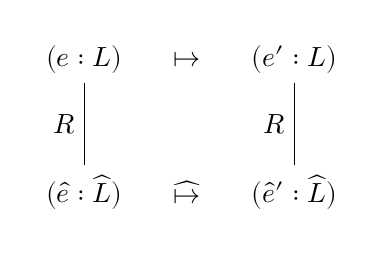
\begin{tikzpicture}[ampersand replacement=\&]

\matrix (m) [matrix of math nodes,row sep=3em,column sep=4em,minimum width=2em]
{ (\Ce : \C) \& (\Ce' : \C) \\
  (\Ae : \A) \& (\Ae' : \A) \\
} ;
\path

(m-1-1) 
edge [white]
node [black] {$\Csteps$} 
(m-1-2)

(m-2-1) 
edge [white]
node [black] {$\Asteps$}
(m-2-2)

(m-1-1) 
edge
node [left] {$R$} 
(m-2-1)

(m-1-2) 
edge
node [left] {$R$} 
(m-2-2)

;

\end{tikzpicture}\end{center}\end{donotbreak}

This picture takes place at some point in the analysis process.
$\Ce$ is the current program (possibly the result of running the base program for a little while).
$\Ae$ is a valid abstraction of $\Ce$, where this validity is expressed some relation $R$ holding between $\Ce$ and $\Ae$.
$\Ce'$ is some next state of execution of $\Ce$, and likewise for $\Ae$/$\Ae'$.
In order to be a correct analysis, it must be guaranteed that $\Ce'$ and $\Ae'$ will be related.
The logical structure of the picture is given by:
\begin{equation*}
∀ (\Ce,\Ce' : \C ) (\Ae,\Ae' : \A), (\Ce R \Ae) ∧ (\Ce \Csteps \Ce') ∧ (\Ae \Asteps \Ae') ⇒  (\Ce' R \Ae')
\end{equation*}

% }}}

% Galois Connections {{{
\subsection{Galois Connections}
\label{section:Background:GaloisConnections}

The AI setting can be elegently simplified and enriched through the use of \emph{galois connections}.
Galois connections serve as a unifying framework for establishing the "relationship between $\C $ and $\A$" mentioned in the previous section.

A galois connection between two posets (sets with a partial order) $\C$ and $\A$ is notated $\C\galois{α}{γ}\A$ and contains:
\begin{itemize}
\item $(α : \C → \A)$ where $α$ is monotonic
\item $(γ : \A → \C )$ where $γ$ is monotonic
\item $(γ ∘ α)$ is expansive: $∀ (x : \C ), x ⊑ γ(α(x))$
\item $(α ∘ γ)$ is contractive: $∀ (y : \A), α(γ(y)) ⊑ y$
\end{itemize}
The last two properties can be succinctly stated as $(α ∘ γ ⊑ id ⊑ γ ∘ α)$\footnote{
  This uses the logical monotonicity relation $f ⊑ g ⇔  (x ⊑ y ⇒  f(x) ⊑ g(y))$ for the function space
}.
Equivalent to all four properties is the property $x ⊑ γ(y) ⇔  α(x) ⊑ y$.

\paragraph{Example:}
Given a galois connection $\C\galois{α}{γ}\A$, there exists a galois connection $\C → \C  \galois{α}{γ} \A → \A$ where:
\begin{align*}
α(f : \C → \C) &≔ γ ∘ f ∘ α \\
γ(g : \A → \A) &≔ α ∘ g ∘ γ \\
\end{align*}

\paragraph{Example:} 
The language $(\PM(ℤ),+,*)$ forms a galois connection with the language $(\PM({EVEN, ODD}),∧,∨)$ where:
\begin{align*}
α(zs : \PM(ℤ))           &≔ ⋃ { { EVEN | ∃ z ∈ zs ∧ Even(z)}, { ODD | ∃ z ∈ zs ∧ Odd(z) } }      \\
γ(ts : \PM({EVEN, ODD})) &≔ ⋃ { { z ∈ ℤ | EVEN ∈ ts ∧ Even(z) }, { z ∈ ℤ | ODD ∈ ts ∧ Odd(z) } } \\
\end{align*}

Galois connections simplify the AI framework by using $x ⊑ γ(y)$ or (equivalently) $α(x) ⊑ y$ as the relation $(x R y)$.
Put differently, galois connections are a natural and general way of placing partial orders \emph{on sets themselves} (note that x and y live in different sets).
One can also think of galois connections as something like an isomorphism, but with a weaker round-trip property.
(An isomorphism would require $α ∘ γ = id = γ ∘ α$.)

Using galois connections, the AI framework introduced in the previous section can be re-stated. In the AI framework, an analysis for $\Ce$ is:
\begin{itemize}
\item 
  An abstract language $\A$.
\item 
  A galois connection $\C\galois{α}{γ}\A$.
\item 
  An abstract version of the $\Csteps$ relation: $(\Asteps : \A × \A → Prop)$
\item 
  A way to explore every state reachable by $\Ae$ under $\Asteps$.
  This often requires $\A$ to be finite.
\end{itemize}
The content of the approach is shown in the following picture:
\begin{donotbreak}
\begin{center}
\begin{tabular*}{0.66\textwidth}{@{\extracolsep{\fill}} c c}

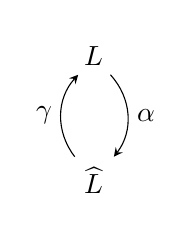
\begin{tikzpicture}[ampersand replacement=\&]
\matrix (m) [matrix of math nodes,row sep=3em,column sep=4em,minimum width=2em]
{ \C \\
  \A \\
} ;
\path [-stealth]

(m-1-1) 
edge [bend left=40]
node [right] {$α$} 
(m-2-1)

(m-2-1) 
edge [bend left=40]
node [left] {$γ$} 
(m-1-1)

;
\end{tikzpicture}

&

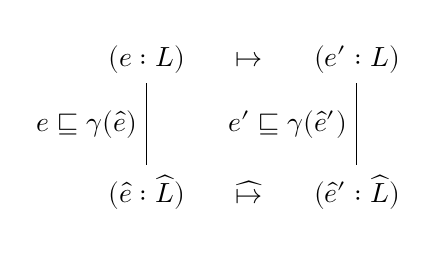
\begin{tikzpicture}[ampersand replacement=\&]
\matrix (m) [matrix of math nodes,row sep=3em,column sep=4em,minimum width=2em]
{ (\Ce : \C) \& (\Ce' : \C) \\
  (\Ae : \A) \& (\Ae' : \A) \\
} ;
\path

(m-1-1) 
edge [white]
node [black] {$\Csteps$} 
(m-1-2)

(m-2-1) 
edge [white]
node [black] {$\Asteps$}
(m-2-2)

(m-1-1) 
edge
node [left] {$\Ce ⊑ γ(\Ae)$} 
(m-2-1)

(m-1-2) 
edge
node [left] {$\Ce' ⊑ γ(\Ae')$} 
(m-2-2)

;
\end{tikzpicture}

\end{tabular*}
\end{center}
\end{donotbreak}

This picture takes place at some point in the analysis process.
$\Ce$ is the current program (possibly the result of running the base program for a little while).
$\Ae$ is a valid abstraction of $\Ce$ by construction as $α(\Ce)$.
$\Ce'$ is some next state of execution of $\Ce$, and likewise for $\Ae$/$\Ae'$.
In order to be a correct analysis, it must be guaranteed that $\Ce' ⊑ γ(\Ae')$.
The logical structure of the picture is given by:
\begin{equation*}
∀ (\Ce,\Ce' : \C ) (\Ae,\Ae' : \A), (\Ce ⊑ γ(\Ae)) ∧ (\Ce \Csteps \Ce') ∧ (\Ae \Asteps \Ae') ⇒  (\Ce' ⊑ γ(\Ae'))
\end{equation*}

The logical structure of the previous figure is the \emph{soundness} property of the analysis.
This property can be simplified further by the statement $\Csteps ⊑ γ(\Asteps)$.
This uses the definition of galois connections for function spaces shown in a previous example.
What is more, this more compact statement of soundness also captures another property, the \emph{tightness} of the analysis.
Unfolded, this property states:
\begin{equation*}
∀ (\Ce,\Ce' : \C ) (\Ae,\Ae' : \A), (\Ce' ⊑ γ(\Ae')) ∧ (\Ce \Csteps \Ce') ∧ (\Ae \Asteps \Ae') ⇒  (\Ce ⊑ γ(\Ae))
\end{equation*}
Tightness tells us that our abstraction is provably \emph{the best abstraction possible}.
The beauty of galois connections is how they capture both soundness and tightness of an analysis with one concise statement: $\Csteps ⊑ γ(\Asteps)$.

% }}}

% CPS {{{
\subsection{Continuation Passing Style}
\label{section:Background:ContinuationPassingStyle}

We use CPS-IF as an example language to demonstrate the benefits of our framework.
CPS is a syntactically restricted version of the lambda calculus.
CPS-IF is an extension of CPS with conditionals.
We choose CPS because the state machine for the semantics of CPS requires no call stack.
We add conditionals to make things slightly more interesting.

We define the CPS-IF language as follows:
\begin{align*}
x,y,k &: Var  &⩴ ..variables..                          \\
b,i,l &: Lit  &⩴ ℤ ⋃ 𝔹                                  \\
f,g   &: Lam  &⩴ λ(x) → c | λ(x,k) → c                  \\
a     &: Atom &⩴ x | l | f | op(a)                      \\
op    &: Op   &⩴ add1 | sub1 | gez                      \\
c     &: Call &⩴ if(a){c}{c} | a(a) | a(a,a) | halt(a)  \\
\end{align*}

CPS-IF supports integer and boolean literals, addition and subtraction by 1, and testing if an integer is greater than or equal to zero.
The essence of CPS is in the syntactic restriction on application forms $a(a)$ and $a(a,a)$.  
Because $a$ cannot be a nested call expression, evaluating a $Call$ requires no evaluation stack.

All lambda calculus terms can be translated to CPS terms through CPS-conversion.
However, because lambda calculus terms are much easier to read, we will use lambda calculus terms for examples.
We display the CPS-converted version of examples where appropriate.

% }}}

% Control Flow Analysis {{{
\subsection{Control Flow Analysis}
\label{section:Background:ControlFlowAnalysis}

Control flow analysis is a class of analysis which is particularly important for higher-order languages.
In non-higher-order languages, it is useful to distinguish control-flow--which functions can be called--from data-flow--which values flow where.
Traditionally one performs a control-flow analysis first, to find out which functions are called, and a data-flow analysis second, using the results of the control flow analysis.

In higher-order languages, data-flow and control-flow become the same problem.
Before you can tell which functions will be called, you need to know how values flow, because functions are themselves values.

We note that the distinction between "higher-order" languages and "non-higher-order" languages is a red herring.
Functions can be passed as values in C using function pointers, and object-oriented languages enjoy a similar circularity between control- and data- flow from method dispatch.
You can read these statements as saying "all languages are higher order, and thus need control flow analysis".
Or you can read them as saying "all languages are higher order, and we've done just fine without control flow analysis so far".
The distinction is in the code that you end up analysing.

We build on the tradition of control flow analysis pioneered by Shivers and its recent refinements developed by Might and Van Horn.
In this tradition, the result of a control flow analysis is closer to what one would think of as a data-flow analysis.
0CFA, the most basic control flow analysis, computes (conservatively) the set of values which might flow to a particular variable.
kCFA is a suite of context sensitive extensions to 0CFA which analyses a given function separately for each possible calling context.
We use 0CFA as the example analysis in this paper.
However our framework, and our implementation of it, scale to the full range of context sensitive control flow analyses.

% }}}

% }}}

% Monadic AAM {{{

\section{Monadic AAM}
\label{section:MonadicAAM}

Monadic AI (Sergey et al. PLDI 2013) showed that computational modularity for abstract interpreters can be achieved through a monadic abstraction.
We build directly on this work at the level of intuition--monads serve as our pivot-point for generalizing abstract control.
However, in our pursuit of an axis-independent correctness framework, our approach deviates greatly from this work in the specific interfaces used.

First we demonstrate a simple 0CFA analysis on CPS-IF which doesn't use our framework.
The language is the same as introduced in section \ref{section:Background:ContinuationPassingStyle}, and repeated here for convenience:
\begin{align*}
x,y,k &: Var  &≔ ..variables..                          \\
b,i,l &: Lit  &≔ ℤ ⋃ 𝔹                                  \\
f,g   &: Lam  &⩴ λ(x) → c | λ(x,k) → c                  \\
a     &: Atom &⩴ x | l | f | op(a)                      \\
op    &: Op   &⩴ add1 | sub1 | gez                      \\
c     &: Call &⩴ if(a){c}{c} | a(a) | a(a,a) | halt(a)  \\
\end{align*}
The abstract semantics of 0CFA will track literals (including lambdas) that appear in the program text.
For integers that do not appear in the program text, the analysis uses a single token $INT$ which conservatively approximates any possible integer.
Because there are a finite many literals in the program text, there are a finite number of possible values.
Formally, the state space for the abstract machine of the abstract semantics is defined as:
\begin{align*}
v &: \AVal   ⩴ INT | l | λ(x) → c | λ(x,k) → c \\
σ &: \AStore ≔ Var → \PM(\AVal)                 \\
Σ &≔ \PM(Call × \AStore)                        \\
\end{align*}

The abstract semantics for $Σ$ comes in two parts.  
First we define a \emph{denotation function} $(𝒜 : \AStore × Atom → \PM(\AVal))$ for $Atom$ expressions.
Second we define a \emph{step relation} (as a function) $(𝒞 : Call × \AStore → \PM(Call × \AStore))$ for $Call$ expressions.
\begin{align*}
𝒜                            &: \AStore × Atom → \PM(\AVal)  \\
𝒜 (σ,x)                      &≔ σ(x)                        \\
𝒜 (σ,l)                      &≔ { l }                       \\
𝒜 (σ,add1 a) | 𝒜 [ρ,σ] ⊑ INT &≔ { INT }                     \\
𝒜 (σ,sub1 a) | 𝒜 [ρ,σ] ⊑ INT &≔ { INT }                     \\
𝒜 (σ,gez a)  | 𝒜 [ρ,σ] ⊑ INT &≔ { T , F }                   \\
𝒜 (σ,λ(x)(k) → c)            &≔ { λ(x)(k) → c }             \\
\end{align*}

% \begin{align*}
% 𝒞                   &: &Call × \AStore → \PM(Call × \AStore)                                     \\
% 𝒞 <if(a){c₁}{c₂},σ> &≔ &{ <c,σ>                                                                 \\
%                     &  &|             c &∈ ⋃ { { c1 } if T ∈ 𝒜 (σ,a), { c2 } if F ∈ 𝒜 (σ,a) }   \\
%                     &  &}                                                                       \\
% 𝒞 <a₁(a₂,a₃),σ>     &≔ &{ <c,σ'>                                                                \\
%                     &  &| <λ(x)(k) → c> &∈ 𝒜 (σ,a₁)                                             \\
%                     &  &|            v₂ &∈ 𝒜 (σ,a₂)                                             \\
%                     &  &|            v₃ &∈ 𝒜 (σ,a₃)                                             \\
%                     &  &|            σ' &≔ σ ⊔ [x ↦ v₂] ⊔ [k ↦ v₃]                              \\
%                     &  &}                                                                       \\
% \end{align*}

The complete analysis of a program c is defined as the least fixed point of a
\emph{collection semantics} for the relation $𝒞$:
\begin{align*}
μ(Σ) → {<c,⊥>} ⊔ 𝒞*(Σ)
\end{align*}
where
\begin{align*}
𝒞*    &: \PM(Call × \AStore) → \PM(Call × \AStore) \\
𝒞*(Σ) &≔ ⋃ { 𝒞 <c,σ> | <c,σ> ∈ Σ }               \\
\end{align*}
(The collecting semantics tracks all states that the program could be in rather than just the final states.)

The first insight in monadic static analysis is to abbreviate the definitions of $𝒜 $ and $𝒞$ using a monad.
At this point, the monad "trick" is nothing more than simplifying the definition. 
This simplification is similar to how a functional programmer would use a state monad in place of explicit state passing.

We use a powerset monad and state monad transformer to write the analysis in monadic style.
The full definitions of the monads used throughout this paper are defered to section \ref{section:Proofs+Definitions}.
Because monad transformers are just fancy names for simple types, we write the simple types underneath definitions which use monad transformers.
The monadic conversion of the above analysis is:
\begin{align*}
ℳ     &: Set → Set                  \\
ℳ (a) &≔ \ST(\AStore)(\PM)(a)       \\
ℳ (a) &≔ \AStore → \PM(a × \AStore) \\
\end{align*}

\begin{align*}
𝒜                &: Atom → ℳ (\PM(\AVal))                    \\
𝒜 (x)            &≔ do                                       \\
                 &σ ← get-σ                                  \\
                 &return(σ(x))                               \\
𝒜 (l)            &≔ return({l})                              \\
𝒜 ₘ(add1(a))     &≔ do                                       \\
                 &v ← 𝒜 (a)                                  \\
                 &return({INT | ∃ i ⊑ INT ∈ v})              \\
𝒜 ₘ(sub1(a))     &≔ do                                       \\
                 &v ← 𝒜 (a)                                  \\
                 &return({INT | ∃ i ⊑ INT ∈ v})              \\
𝒜 ₘ(gez(a))      &≔ do                                       \\
                 &v ← 𝒜 (a)                                  \\
                 &return(⋃ { {T, F} | ∃ i ⊑ INT ∈ v})        \\
𝒜 ₘ(λ(x)(k) → c) &≔ return({λ(x)(k) → c})                    \\
                                                             \\
𝒞                 &: Call → ℳ (Call)                         \\
𝒞 (if(a){c₁}{c₂}) &≔ do                                      \\
                  &vP ← 𝒜 (a)                                \\
                  &v ← lift\PM(vP)                           \\
                  &b ← coerce𝔹(v)                            \\
                  &return { if b then c₁ else c₂ }           \\
𝒞ₘ(a₁(a₂,a₃))     &≔ do                                      \\
                  &vP ← 𝒜 (a₁)                               \\
                  &v ← lift\PM(vP)                           \\
                  &<λ(x)(k) → c> ← coerceλ₂(v)               \\
                  &vP₂ ← 𝒜 (a₂)                              \\
                  &vP₃ ← 𝒜 (a₃)                              \\
                  &v₂ ← lift\PM(vP₂)                         \\
                  &v₃ ← lift\PM(vP₃)                         \\
                  &modify-σ (λ(σ) → σ ⊔ [x ↦ v₂] ⊔ [k ↦ v₃]) \\
                  &return(c)                                 \\
\end{align*}

The monadic abstraction provides a nice way to simplify the implementation of the analysis.  
In particular, cases which do not modify the store or only return one result.
Both of these cases are instances of having "no effect", and they need not mentioned all members of the state machine.  
(This was observed in Sergey et. al. PLDI 2013.)

As before, we must complete the analysis by building an abstract machine transition function:
\begin{align*}
𝒞*    &: \PM(Call × \AStore) → \PM(Call × \AStore) \\
𝒞*(Σ) &≔ ⋃ { (𝒞ₘ c)(σ) | <c,σ> ∈ Σ }               \\
\end{align*}

The monad we used recovers exactly the analysis we wrote before.
On top of the convenience of writing things monadically, our insight and contribution is twofold:
\begin{itemize}
\item ℳ  can be \emph{axiomatized}, such that different definitions for ℳ  give rise to different control abstractions for the analysis.
\item The monadic abstraction provides for a modular proof framework for establishing the correctness of the analysis.
\end{itemize}

% }}}

% Abstract Control {{{
\section{Abstract Control}
\label{section:AbstractControl}

The current instantiation of ℳ  yields a flow-sensitive path-sensitive analysis.  
Consider a reordering of the powerset\footnote{
  The definition of $\PT$ we use is non-traditional.  However, our definition
  for $\PT$ is actually a monad, whereas traditional definitions are not.  Our
  definition and proofs for $\PT$ are given in section \ref{section:Proofs+Definitions}.
}
and state monad transformers:
\begin{align*}
ℳ     &: Set → Set                  \\
ℳ (a) &≔ \PT(\SM(\AStore))(a)       \\
ℳ (a) &≔ \AStore → \PM(a) × \AStore \\
\end{align*}

As before, we must convert between monadic actions and abstract state space transitions to achieve an analysis:
\begin{align*}
𝒞*       &: \PM(Call) × \AStore → \PM(Call) × \AStore                          \\
𝒞*<cP,σ> &≔ <{c' | c' ∈ π₁(𝒞(c))(σ) | c ∈ c\PM }, ⋃ { π₂(𝒞(c))(σ) | c ∈ cP }>  \\
\end{align*}
This instantiation of $ℳ $ and $𝒞*$ yields a flow-insensitive analysis.

For the same monad $ℳ $, we can change the definition of $𝒞*$ to achieve a flow-sensitive path-insensitive analysis:
\begin{align*}
𝒞*    &: \PM(Call × ^Store^) → \PM(Call × ^Store^)           \\
𝒞*(Σ) &≔ { <c',π₂(𝒞(c))(σ)> | c' ∈ π₁(𝒞(c))(σ) | <c,σ> ∈ Σ } \\
\end{align*}

In the correctness framework, both the flow-sensitive path-sensitive analysis and flow-insensitive analyses are justified through isomorphisms between monadic actions and abstract state space transitions.  
The flow-sensitive path-insensitive variant is recovered by weakening this isomorphism to a galois connection.

% }}}

% Intensional Optimizations {{{

\section{Intensional Optimizations}
\label{section:IntensionalOptimizations}

Up to this point we have factored the abstract control properties of static analysis behind a common interface.  
Now we show how to implement two intentional optimizations, abstract garbage collection and mcfa, in a completely general setting.

The common interface for each variation in abstract control is a monad $ℳ  ∈ Set → Set$ with $get$, $put$, and nondeterminism effects.
We abreviate the conjunction of the above properties holding on some ℳ  as $Analysis(ℳ )$.

\paragraph{Abstract Garbage Collection}
Abstract garbage collection is a technique in abstract interpretation where unreachable abstract adresses are pruned from the state space.
This is analagous to "real" garbage collection, where unreachable pointers are reclaimed for space efficiency.
However, in abstract semantics, adresses are \emph{re-used} to soundly and finitely aproximate an infinite address space.
Impreceision in control flow analyses arise when an abstract address present in the current store must be used for allocation.
Abstract garbage collection is a purely precision and performance improving optimization which removes unreachable abstract adresses.

We will use our generic monadic interfact $Analysis(ℳ )$ for an arbitrary monad $ℳ $.
Using this interface, abstract garbage collection can be implemented once in a purely generic way.
\begin{align*}
gc    &: Call → ℳ (1)                                      \\
gc(c) &≔ do                                                \\
      &σ ← get-σ                                           \\
      &𝓉₀ ← 𝓉-𝒞(c)                                         \\
      &let 𝓉 ≔ μ(𝓉) → 𝓉 ⊔ 𝓉-Var(𝓉)                         \\
      &modify-σ (λ(σ) → ⋃ { [x ↦ v] | x ∈ 𝓉 ∧ σ(x) = v } ) \\
\end{align*}
This is literally the implementation of \emph{concrete} garbage collection.
However, it seamlessly becomes abstract garbage collection when instantiated with the appropriate monad.

\paragraph{MCFA}
MCFA is an optimization that improves the asymptotic complexity of context-sensitive control flow analyses.
kCFA explodes exponentially for $k > 0$ in functional analyses, causing extremely poor analysis performance in the worst case.
However, an apparent paradox was discovered as kCFA was proven to be polynomial in the worst case for object-oriented programs.
MCFA resolved the paradox by identifying the difference in analyses and transfering the polynomial behavior to functional analysis.
The crux of MCFA is to create packed, copied closures rather than linked closures.

So far, our analysis has not used closures for abstract values; 0CFA only tracks lambdas without their closing context.
Adding closures to abstract values is a straightforward addition to the examples we've shown.
Also, our implementation implements all of these features in their full glory.

The mcfa optimization of copying rather than linking closures similarly enjoys a fully generic implementation:
\begin{align*}
clo-copy       &: [Var] × Call → ℳ (Clo)             \\
clo-copy(xs,c) &≔ do                                 \\
               &let ys ≔ free-vars(c)                \\
               &σ ← get-σ                            \\
               &vs ← map* σ ys                       \\
               &ρ ← { y ↦* v | (y,v) ∈ zip(ys, vs) } \\
               &return <xs,c,ρ>                      \\
\end{align*}

Using existing techniques, these optimizations would need to be both implemented and proven correct for each instantiation of abstract control.
Our generalization over abstract control allows us to implement each of these optimizations once.
More importantly, the proofs about these optimizations need only happen once as well, and the proofs transfer to their instantiations for free.

% }}}

% Correctness Framework {{{

\section{Correctness}
\label{section:Correctness}

The key advantage to our framework is that the proofs of correctness for constructed analyses are derived automatically.

We must now relate monadic actions like 𝒞 back to small step semantics.
To do this we establish a galois connection between monadic actions in ℳ  and transitions functions for \emph{some} abstract state space $𝒮𝒮$.
This abstract state space is constructed from the monad transformer stack, however some transformer stacks support multiple abstract state spaces.
This step is notated $(A → ℳ (B))\galois{α}{\gamma}(𝒮𝒮(A) → 𝒮𝒮(B))$.
We call a particular monad $ℳ $ which enjoys this property a \emph{small-step monad}.

In our framework we prove that not only are $\ST$ and $\PT$ monad transformers, they're small-step monad transformers.
This means that for any stack of interleaving $\ST$ and $\PT$ monad transformers, one can construct the needed galois connection.

In our framework we prove that $\ST(𝓈)(\PM) ⊑ \PT(\SM(𝓈))$.
These monad interleavings correspond to path-sensitivity and path-insensitivity respectively.

In our framework we prove that for the $\PT(\SM(𝓈))$ monad, two galois connections are possible to the state space $\PM(\_ × 𝓈)$.
These choices for galois connection correspond to flow-sensitivity and flow-insensitivity respectively.

Independent of language or application, we can now conclude abstractly (yet precisely):
\begin{align*}
flow-insensitive ⊑ flow-sensitive path-insensitive ⊑ flow-sensitive 
\end{align*}

When using our framework, the analysis designer need only prove prove:
\begin{itemize}
\item The semantic step function 𝒞 (which calls 𝒜 ) is monotonic, including monotonic in the choice of 𝓂 .
\item The semantics as written, including intensional optimizations, are correct.
\end{itemize}
After supplying these proofs, the analysis designer enjoys:
\begin{itemize}
\item An automatically derived analysis for their language with their choice of abstract control.
\item A proof-by-construction of correctness for the derived analysis.
\item Seamless extensions to AAM and intensional optimizations (like gc or mcfa).
\end{itemize}

Our proof technique is maximally modular in that new monads can be composed seamlessly into the framework with disruption.
This modularity greatly reduces the proof burden on the analysis designer as new languages and analyses are developed.

In practice, there will be many more state space components, like abstract time and abstract address in the AAM framework.
To add these features, the analysis designer need only stack more state space monads together to augment the resulting abstract state machine.
However, once monotonicity of the $𝒞$ action is established, both concrete and abstract interpreters can be derived for free.
This is only possible because all proofs have been decomposed to the unit of monad transformer.

% }}}

% Proofs and Definitions {{{

\section{Proofs and Definitions}
\label{section:Proofs+Definitions}

This section details all structures used in this paper and their proofs.

% Setup {{{

\subsection{Setup}
\label{section:Proofs+Definitions:Setup}

\begin{verbatim}
PartialOrder(A : Set) ≔
  operators
    ⊑ : A → A → Prop
  laws
    reflexivity : x ⊑ x
    antisymmetry : x ⊑ y ⇒  y ⊑ x ⇒  x = y
    transitivity : x ⊑ y ⇒  y ⊑ z ⇒  x ⊑ z
\end{verbatim}

\begin{verbatim}
Monotonic(𝑓 : A → B) ≔ 
  require
    PartialOrder(A)
    PartialOrder(B)
    ∀ (x y : A), x ⊑ y ⇒  f(x) ⊑ f(y)
\end{verbatim}

\begin{verbatim}
(C : Set) α⇄ γ (A : Set) ≔
  require
    PartialOrder(C)
    PartialOrder(A)
  operators
    α : C → A
    γ : A → C
  laws
    Monotonic(α)
    Monotonic(γ)
    α ∘ γ ⊑ id ⊑ γ ∘ α
\end{verbatim}

\begin{verbatim}
JoinSemilattice(A : Set) ≔
  require
    PartialOrder(A)
  operators
    ⊥ : A
    ⊔ : A → A → A
  laws
    left-unit : ⊥ ⊔ x = x
    right-unit : x ⊔ ⊥ = x
    associativity : x ⊔ (y ⊔ z) = (x ⊔ y) ⊔ z
    commutativity : x ⊔ y = y ⊔ x
\end{verbatim}

\begin{verbatim}
Monad(𝓂  : Set → Set) ≔
  operators
    return : ∀ (A : Set) → A → 𝓂 (A)
    extend : ∀ (A B : Set) → (A → 𝓂 (B)) → (𝓂 (A) → 𝓂 (B))
  laws
    left-unit : extend(return) = id
    right-unit : extend(k)(return(A)) = k(A)
    associativity : extend(k₂)(extend(k₁)(aM)) = extend(λ x → extend(k₂)(k₁(x)))(A)
\end{verbatim}

\begin{verbatim}
Transformer(𝒯 : (Set → Set) → (Set → Set)) ≔
  require
    ∀ (𝓂  : Set), Monad(𝓂 ) ⇒  Monad(𝒯(𝓂 ))
  operators
    lift : ∀ (𝓂  : Set), 𝓂 (A) → 𝒯(𝓂 )(A)
  laws
    unit : lift(return) = return
\end{verbatim}

\begin{verbatim}
MonadState(𝓈 : Set)(𝓂  : Set → Set) ≔
  operators
    get : 𝓂  𝓈
    put : 𝓈 → 𝓂  1
\end{verbatim}

\begin{verbatim}
MonadPlus(𝓂  : Set → Set) ≔ 
  require
    ∀ (A : Set), JoinSemilattice(𝓂 (A))
  laws
    left-zero : extend(k)(⊥) = ⊥
    right-zero : extend(const(⊥))(aM) = ⊥
    distributivity : extend(k)(aM₁ ⊔ aM₂) = extend(k)(aM₁) ⊔ extend(k)(aM₂)
\end{verbatim}

\begin{verbatim}
Functorial(ℭ : Set → Prop)(𝓂  : Set → Set) ≔ 
  require
    ∀ (A : Set), ℭ (A) → ℭ (𝓂 (A))
\end{verbatim}

\begin{verbatim}
Pointed(𝓂  : Set → Set) ≔
  unit : ∀ (A : Set) → A → 𝓂 (A)
\end{verbatim}

\begin{verbatim}
MonadSmallStep(𝓂  : Set → Set)(𝒮𝒮 : Set → Set) ≔ 
  require
    ∀ (A B : Set), (A → 𝓂 (B)) α⇄ γ (𝒮𝒮(A) → 𝒮𝒮(B))
\end{verbatim}

% }}}

% SetT {{{
\subsection{\ST}
\label{section:Proofs+Definitions:SetT}

\begin{verbatim}
\ST : (Set → Set) → (Set → Set)
\ST(𝓂 )(A) ≔ 𝓂 (\PM(A))

-----------------
Transformer(\ST)

lift : ∀ (𝓂  : Set → Set) (A : Set), 𝓂 (A) → \ST(𝓂 )(A)
lift ≔ map (λ x → { x })

Monad(𝓂 ) ∧ Functorial(JoinSemilattice)(𝓂 )
-------------------------------------------
Monad(\ST(𝓂 ))

return : ∀ (A : Set), A → \ST 𝓂  A
return ≔ lift ∘ returnₘ

extend : ∀ (A B : Set), (A → \ST(𝓂 )(B)) → (\ST(𝓂 )(A) → \ST(𝓂 )(B))
extend(k) ≔ joinₘ ∘ mapₘ (joins ∘ mapₚ k)

Monad(𝓂 ) ∧ Functorial(JoinSemilattice)(𝓂 )
-------------------------------------------
MonadPlus(\ST(𝓂 ))

m0 : ∀ (A : Set), \ST 𝓂  A
m0 ≔ ⊥ ₘ

<+> : ∀ (A : Set) → \ST 𝓂  A → \ST 𝓂  A → \ST 𝓂  A
<+> ≔ ⊔

Monad(𝓂 ) ∧ MonadState(𝓈)(𝓂 )
-----------------------------
MonadState(𝓈)(𝓂 )

get : \ST 𝓂  𝓈
get ≔ lift getₘ

put : 𝓈 → \ST 𝓂  1
put ≔ lift ∘ putₘ

MonadSmallStep(𝓂 )(𝒮𝒮) ∧ Functorial(JoinSemilattice)(𝓂 ) ∧ Functor(𝒮𝒮)
-------------------------------
MonadSmallStep(\ST 𝓂 )(𝒮𝒮 ∘ \PM)

α : ∀ (A B : Set), (A → \ST(𝓂 )(B)) → (𝒮𝒮(\PM(A)) → 𝒮𝒮(\PM(B)))
α(f) ≔ αₘ(joinsₘ ∘ mapₚ(f))

γ : ∀ (A B : Set), (𝒮𝒮(\PM(A)) → 𝒮𝒮(\PM(B))) → (A → \ST(𝓂 )(B))
γ(f) ≔ γₘ(f ∘ mapₛₛ(unitₚ))

MonadSmallStep(𝓂 )(𝒮𝒮) ∧ (\PM ∘ 𝒮𝒮) α⇄ γ (𝒮𝒮 ∘ \PM)
-------------------------------------
MonadSmallStep(\ST 𝓂 )(\PM ∘ 𝒮)

α : ∀ (A B : Set), (A → \ST(𝓂 )(B)) → (\PM(𝒮𝒮(A) → \PM(𝒮𝒮(B))))
α(f) ≔ extendₚ(α ∘ αₘ(f))

γ : ∀ (A B : Set), (\PM(𝒮𝒮(A) → \PM(𝒮𝒮(B)))) → (A → \ST(𝓂 )(B))
γ(f) ≔ extendₚ(γ ∘ γₘ(f))
\end{verbatim}

% }}}

% StateT {{{

\subsection{$\ST$}
\label{section:Proofs+Definitions:StateT}

\begin{verbatim}
\ST : Set → (Set → Set) → (Set → Set)
\ST(𝓈)(𝓂 )(A) ≔ 𝓈 → 𝓂  (A × 𝓈)

Transformer(\ST(𝓈))
----------------------

lift : ∀ (𝓂  : Set → Set) (A : Set), 𝓂  a → \ST(𝓈)(𝓂 )(A)
lift aM ≔ λ 𝓈 → mapₘ (,𝓈) aM

Monad(𝓂 )
--------------------
Monad(\ST(𝓈)(𝓂 ))

return : ∀ (A : Set), A → \ST(𝓈)(𝓂 )(A)
return ≔ lift ∘ returnₘ

extend : ∀ (A B : Set), (A → \ST(𝓈)(𝓂 )(B)) → (\ST(𝓈)(𝓂 )(A) → \ST(𝓈)(𝓂 )(B))
extend(k)(aM) ≔ λ 𝓈 → doₘ
  (a,𝓈') ← aM(𝓈)
  k(a)(𝓈')

JoinSemilattice(𝓈) ∧ Monad(𝓂 )
------------------------------------------
Functorial(JoinSemilattice)(\ST(𝓈)(𝓂 ))

bot : \ST(𝓈)(𝓂 )(A)
bot ≔ λ(𝓈)→ (⊥ ₛ, ⊥ ₐ)

⊔ : \ST(𝓈)(𝓂 )(A) → \ST(𝓈)(𝓂 )(A) → \ST(𝓈)(𝓂 )(A)
aM₁ ⊔ aM₂ ≔ λ 𝓈 → doₘ
  (a₁,𝓈₁) ← aM₁
  (a₂,𝓈₂) ← aM₂
  return (a₁ ⊔ a₂, 𝓈₁ ⊔ 𝓈₂)

MonadPlus(𝓂 )
------------------------
MonadPlus(\ST(𝓈)(𝓂 ))

⊥ : ∀ (A : Set), \ST(𝓈)(𝓂 )(A)
⊥ ≔ lift ⊥ ₘ

⊔ : ∀ (A : Set), \ST(𝓈)(𝓂 )(A)
aM₁ ⊔ aM₂ ≔ λ 𝓈 → aM₁(𝓈) <+> aM₂(𝓈)

Monad(𝓂 )
----------------------------
Monad\ST(𝓈)(\ST(𝓈)(𝓂 ))

get : \ST 𝓈 𝓂  𝓈
get ≔ λ 𝓈 → return (𝓈,𝓈)

put : 𝓈 → \ST 𝓈 𝓂  1
put(𝓈) ≔ λ (𝓈') → return (∙,𝓈)

MonadSmallStep(𝓂 )(𝒮𝒮)
--------------------------------------
MonadSmallStep(\ST(𝓈)(𝓂 ))(𝒮𝒮(\_ × 𝓈))

α : ∀ (A B : Set), (A → \ST(𝓈)(𝓂 )(B)) → (𝒮𝒮(A × 𝓈) → 𝒮𝒮(B × 𝓈))
α(f) ≔ αₘ (λ (a,𝓈) → f(a)(𝓈))

γ : ∀ (A B : Set), (𝒮𝒮(A × 𝓈) → 𝒮𝒮(B × 𝓈)) → (A → \ST(𝓈)(𝓂 )(B))
γ(f) ≔ λ(a,𝓈) → γₘ (f)(a,s)
\end{verbatim}

% }}}

% Propositions {{{

\section{Propositions}
\label{section:Proofs+Definitions:Propositions}

\begin{itemize}
\item $\PT$ and $\ST$ are Galois Functors.
\item $\PT$ and $\ST$ are MonadStep Functors.
\item 𝒜  and 𝒞 are monotonic (including in 𝓂 ).
\end{itemize}

% }}}

% }}}

% Bibliography {{{
\bibliography{davdar}{}
\bibliographystyle{plain}
% }}}

\end{document}
